\subsubsection{Net 4}
 
\zadatak Proveri kada va{\zv}i
$$
\log_{\frac{x+4}2} \left( \log_2 \frac{2x-1}{3+x} \right) < 0.
$$

\resenje
Da bi prvi logaritam bio definisan mora da va{\zv}i
$$
\frac{x+4}2>0 \land \frac{x+4}2\ne 1 \sledi
x>-4 \land x\ne -2,
$$
a kako vrednost binarnog logaritma mora biti pozitivna, onda argument mora biti
$$
\frac{2x-1}{3+x} >1\sledi x<-3 \lor x>4.
$$
$$
\slika{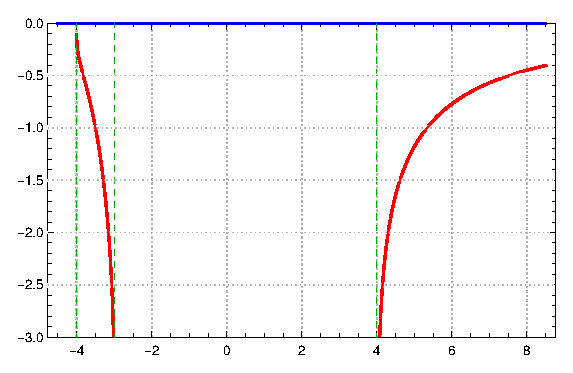
\includegraphics[width=80mm]{eps/4.eps}}{$y=\displaystyle{\log_{\frac{x+4}2} \left( \log_2 \frac{2x-1}{3+x} \right)}$.}
$$
Re{\sv}e{\nj}e  je
$$
x \in \ram{(-4, -3) \cup ( 4, \infty )}.
$$
